\section{REST API}

A REST API is an application programming interface that conforms to the constraints of the REST 
architectural style and allows for interaction with RESTful web services.

REST is not a standard, but rather a set of recommendations and constraints for 
RESTful web services. These include:

\begin{enumerate}
    \item \textbf{Client-Server.} System ‘A’ makes an HTTP request to a URL hosted by 
    System ‘B’, which returns a response.
    It is identical to how a browser works: The application first makes a request 
    for a specific URL, the request is then routed to a web server that returns an HTML page. 
    This page may contain references to images, style sheets, and JavaScript, 
    which incur further requests and responses.

    \item \textbf{Stateless.} REST is stateless: the client request should contain all the 
    information necessary to respond to a request. In other words, it should be possible to
    make two or more HTTP requests in any order and the same responses will be received.

    \item \textbf{Cacheable.} A response should be defined as cacheable or not.
    
    \item \textbf{Layered.} The requesting client need not know whether it’s communicating 
    with the actual server, a proxy, or any other intermediary.~\cite{DevelopersRestAPI}
\end{enumerate}

The working first involves sending a request from the client to the server in the form of web URLs, 
using the HTTP GET, POST, PUT or DELETE methods. After that a response is retrieved from the server 
in the form of a resource which can be anything like HTML, XML, Image or JSON.~\cite{WhatisRESTAPI}

\begin{figure}
    \begin{center}
        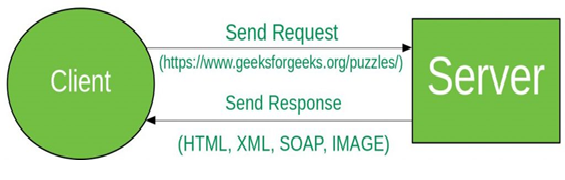
\includegraphics[width=8cm]{restapi.png}
    \end{center}
    \caption{A simple illustration of a REST API request-response.}
    \label{fig:restapi}
\end{figure}

In HTTP there are five methods which are commonly used in a REST based Architecture 
i.e. POST, GET, PUT, PATCH, and DELETE. These methods correspond to create, read, 
update, and delete (or CRUD) operations respectively.~\cite{GeeksRestAPI}

\section{GraphQL}

GraphQL is a query language and server-side runtime for Application Programming Interfaces (APIs) 
that prioritizes giving clients exactly the data they request and nothing more. 
GraphQL is designed to make APIs fast, flexible, and developer-friendly. It is not tied 
to any specific database or storage engine and is instead backed by your existing code and data.

API developers use GraphQL to create a schema to describe all the possible data that clients can query 
through that service. This schema is made up of object types, which define which kind of object you can 
request and what fields it has. As queries come in, GraphQL validates the queries against the schema. 
GraphQL then executes the validated queries.

The API developer attaches each field in a schema to a function called a resolver. 
During execution,the resolver is called to produce the value.~\cite{WhatisGraphQL}

GraphQL follows the same set of constraints as REST APIs, but it organizes data into a 
graph using one interface. Objects are represented by nodes (defined using the GraphQL schema), 
and the relationship between nodes is represented by edges in the graph. Each object is then backed 
by a resolver that accesses the server’s data.

When a GraphQL server responds to an end user’s request, it begins with the query root,
and the resolver executes every field on the requested object. A key-value map houses each field’s
values, and some return another object selecting another set of fields. This continues until only a 
string or a number is returned. The server then responds with a nested set of objects, as requested by 
the end user.~\cite{RubrikGraphQL}

\begin{figure}
    \begin{center}
        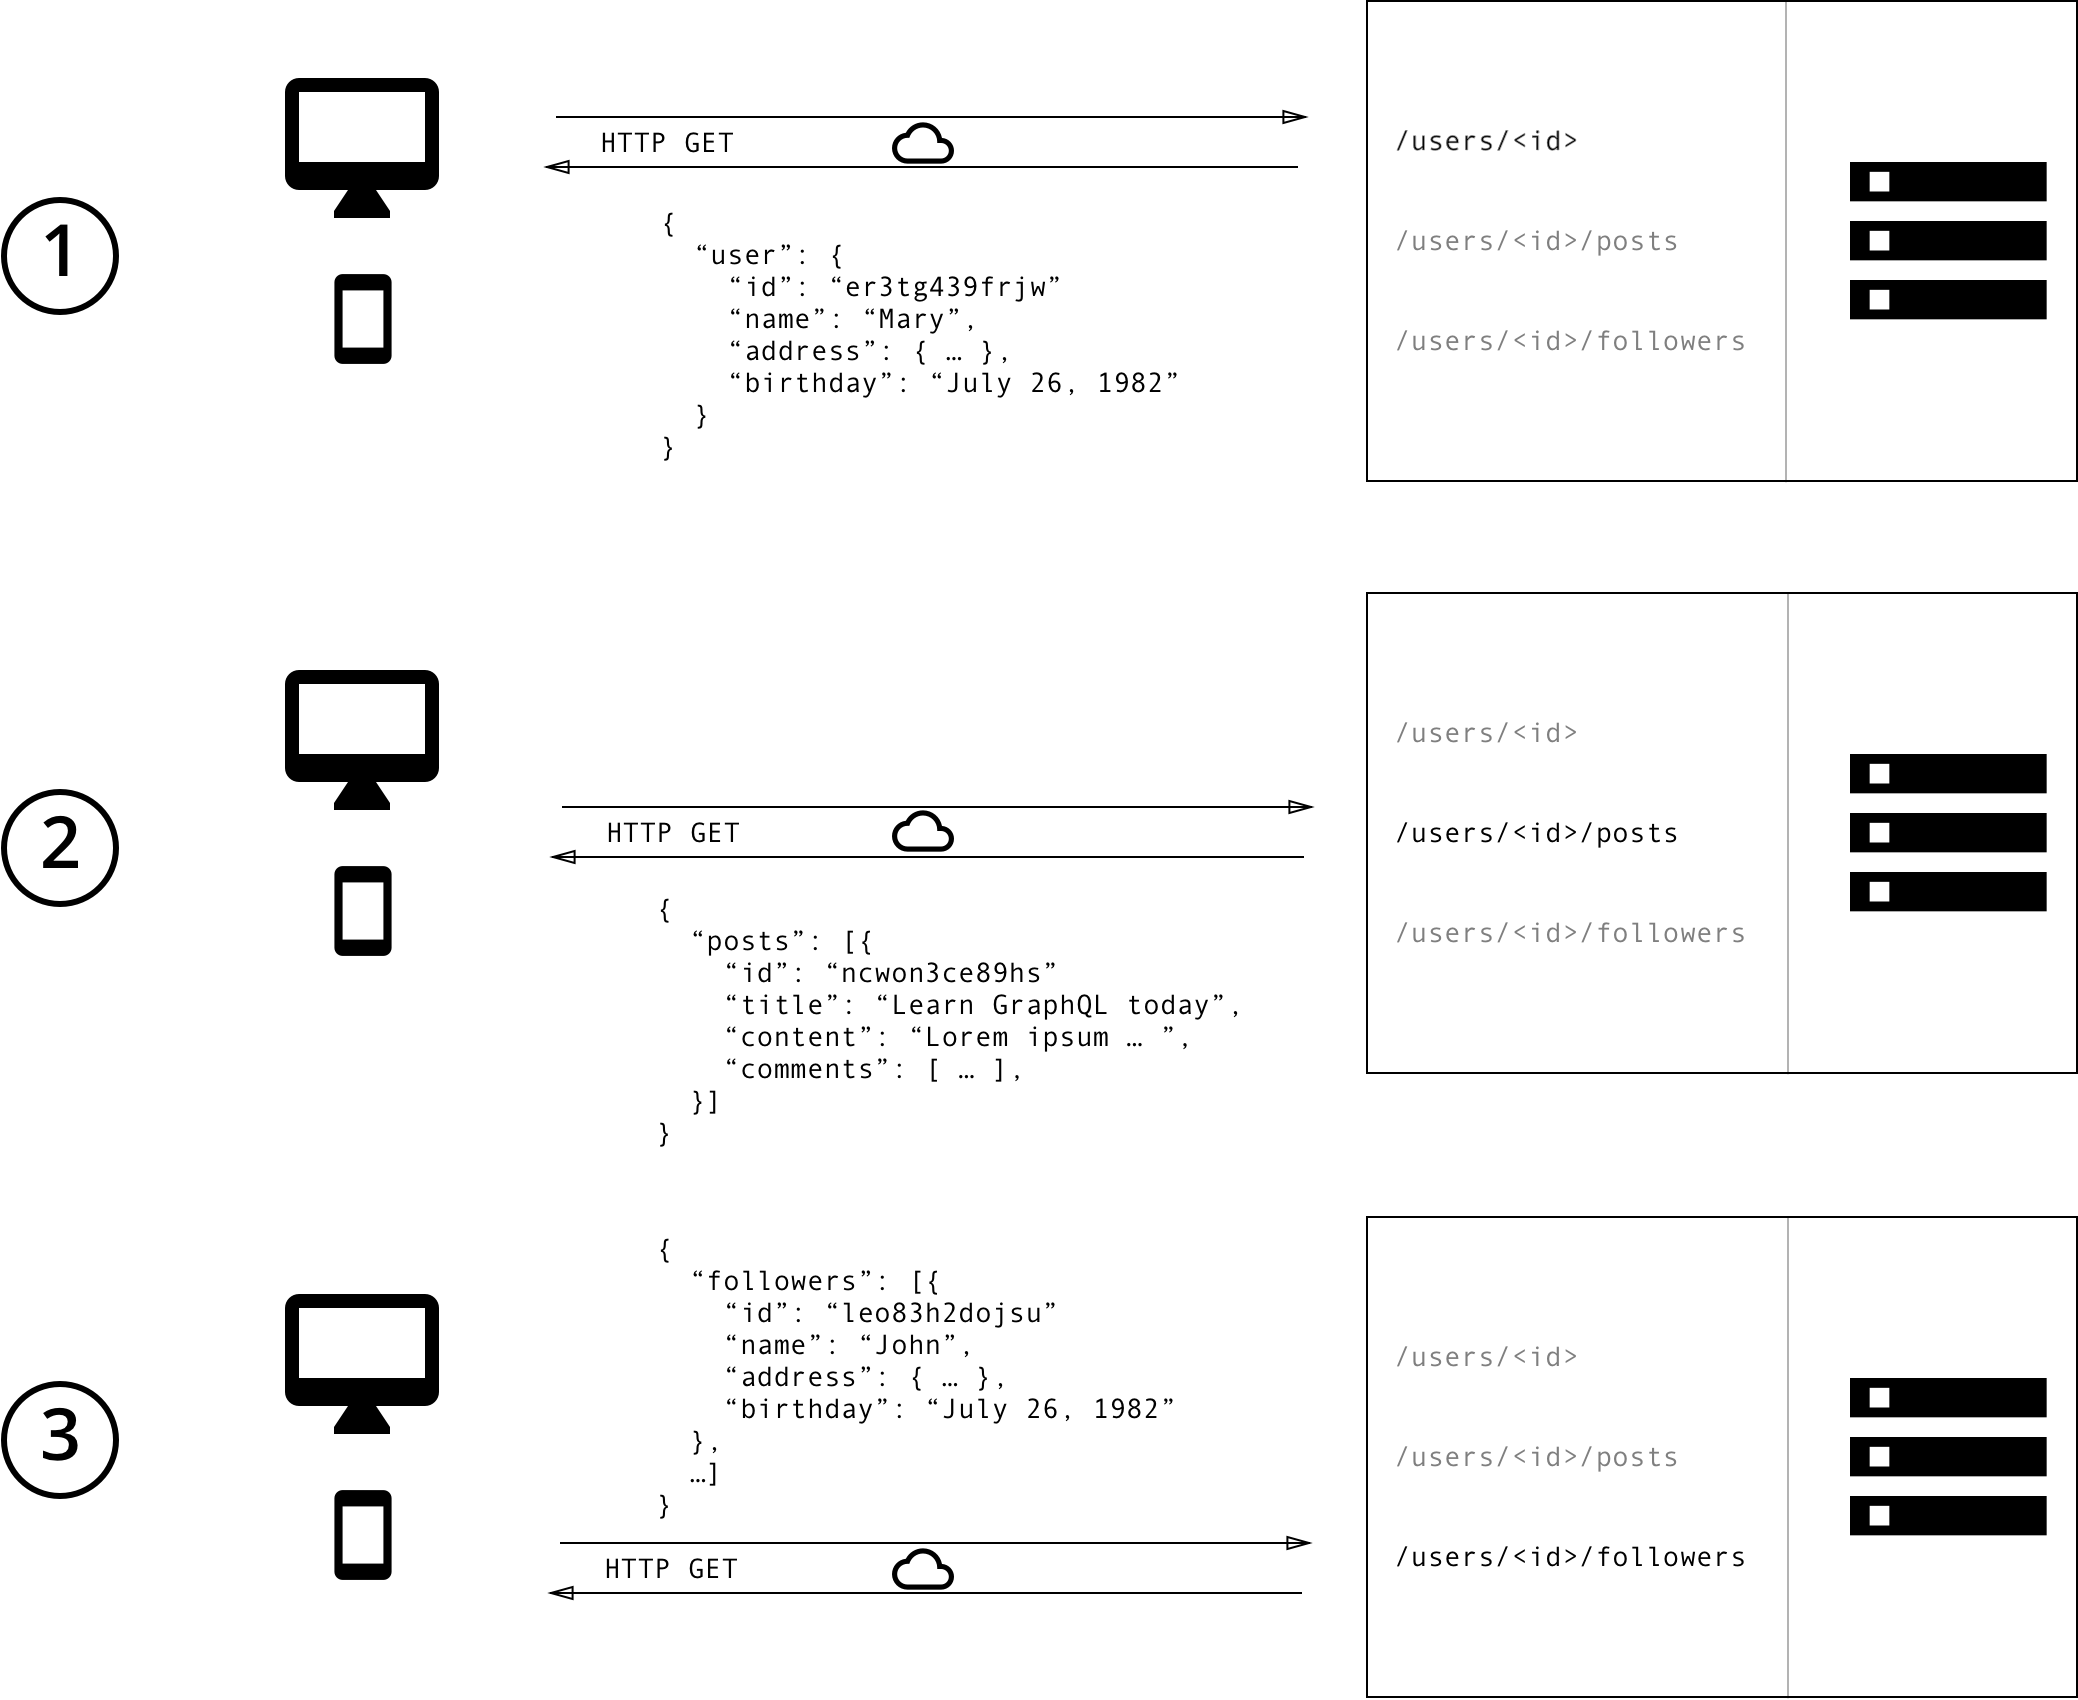
\includegraphics[width=15cm]{graphql-rest.png}
    \end{center}
    \caption{GraphQL can handle the tasks of multiple REST endpoints, 
    neither overfetching, nor underfetching,
    offering the exact data format as requested by the client.~\cite{GraphQLvsREST}}
    \label{fig:graphql}
\end{figure}
  
\subsection{How does GraphQL excel REST API?}

\subsubsection{Data Fetching}

With a REST API, you would typically gather the data by accessing multiple endpoints. You basically 
end up having to make multiple requests to different endpoints to fetch the required data.
In GraphQL on the other hand, you’d simply send a single query to the GraphQL server that 
includes the concrete data requirements. The server then responds with a JSON object where these 
requirements are fulfilled. Therefore using GraphQL, the client can specify exactly the data it needs in a query.

\subsubsection{Over-fetching and Under-fetching of Data}

One of the most common problems with REST is that of over-fetching and under-fetching. This happens 
because the only way for a client to download data is by hitting multiple endpoints that return fixed data structures.
GraphQL gives the clients the exact data they request for.

\subsubsection{Benefits of a Schema and Type System}

GraphQL uses a strong type system to define the capabilities of an API. All the types that are exposed in an API 
are written down in a schema using the GraphQL Schema Definition Language (SDL). This schema serves as the contract 
between the client and the server to define how a client can access the data.
Once the schema is defined, the teams working on frontend and backends can do their work without further communication 
since they both are aware of the definite structure of the data that’s sent over the network.
Frontend teams can easily test their applications by mocking the required data structures. Once the server is ready, 
the switch can be flipped for the client apps to load the data from the actual API.

\subsubsection{Rapid Product Iterations on the Front-end}

A common pattern with REST APIs is to structure the endpoints according to the views that you have inside your app 
in order for the client to get all required information for a particular view by simply accessing the corresponding 
endpoint. However, the major drawback of this approach is that it doesn’t allow for rapid iterations on the frontend. 
With every change that is made to the UI, there is a high risk that now there is more or less data required than before.
Consequently, the backend needs to be adjusted as well to account for the new data needs. This notably slows down the 
ability to incorporate user feedback into a product. But owing to the flexible nature of GraphQL, changes on the 
client-side can be made without any extra work on the server. Since clients can specify their exact data requirements, 
no backend adjustments are required when the design and data needs on the frontend change.

\subsubsection{Insightful Analytics on the Back-end}

GraphQL allows you to have fine-grained insights about the data that’s requested on the backend. As each client specifies 
exactly what information it’s interested in, it is possible to gain a deep understanding of how the available data is being 
used. This can for example help in evolving an API and deprecating specific fields that are not requested by any clients any more.
With GraphQL, you can also do low-level performance monitoring of the requests that are processed by your server. 
GraphQL uses the concept of resolver functions to collect the data that’s requested by a client. Instrumenting and measuring 
performance of these resolvers provides crucial insights about bottlenecks in your system.~\cite{GraphQLvsREST}
